\documentclass[conference]{IEEEtran}
\usepackage{cite}
\usepackage{amsmath,amssymb,amsfonts}
\usepackage{algorithmic}
\usepackage{algorithm}
\usepackage{graphicx}
\usepackage{textcomp}
\usepackage{xcolor}
\usepackage{hyperref}
\usepackage{multirow}
\usepackage[space]{grffile}
\usepackage{array}

\usepackage{placeins} % <--- REQUIRED FOR FIXING THE FLOAT ISSUE
\usepackage{float}    % Required for [H] placement

\def\BibTeX{{\rm B\kern-.05em{\sc i\kern-.025em b}\kern-.08em
    T\kern-.1667em\lower.7ex\hbox{E}\kern-.125emX}}

% --- CUSTOM AUTHOR BREAK ---
\makeatletter
\newcommand{\linebreakand}{%
  \end{@IEEEauthorhalign}
  \hfill\mbox{}\par
  \mbox{}\hfill\begin{@IEEEauthorhalign}
}
\makeatother

\begin{document}

% ==========================
% TITLE
% ==========================
\title{Synapse: A Multimodal Assistive Reading System with Cognitive Difficulty Prediction}

% ==========================
% AUTHORS
% ==========================
\author{
    % --- Professor (Top Center) ---
    \IEEEauthorblockN{1\textsuperscript{st} Ms. Bhanu Verma}
    \IEEEauthorblockA{
    \textit{Asst. Professor, Dept. of CS}\\
    \textit{IMS Engineering College}\\
    Ghaziabad, India\\
    bhanu.verma@imsec.ac.in}
    \and

    \IEEEauthorblockN{2\textsuperscript{nd} Ms. Monika Nagar}
    \IEEEauthorblockA{
    \textit{Asst. Professor, Dept. of CS}\\
    \textit{IMS Engineering College}\\
    Ghaziabad, India\\
    Monika.nagar6@gmail.com}
    \linebreakand

    % --- Students Row ---
    
    \IEEEauthorblockN{3\textsuperscript{rd} Arpit Kumar}
    \IEEEauthorblockA{
    \textit{Dept. of CSE--AIML}\\
    \textit{IMS Engineering College}\\
    Ghaziabad, India\\
    arpitkumar.py@gmail.com}
    \and

    \IEEEauthorblockN{4\textsuperscript{th} Khushi Agarwal}
    \IEEEauthorblockA{
    \textit{Dept. of CSE--AIML}\\
    \textit{IMS Engineering College}\\
    Ghaziabad, India\\
    khushiagarwal192004@gmail.com}
    \and

    \IEEEauthorblockN{5\textsuperscript{th} Anirudh Singh Tomar}
    \IEEEauthorblockA{
    \textit{Dept. of CSE--AIML}\\
    \textit{IMS Engineering College}\\
    Ghaziabad, India\\
    anirudhsinghtomar10@gmail.com}
}

\maketitle

% ==========================
% ABSTRACT
% ==========================
% ==========================
% ABSTRACT
% ==========================

\begin{abstract}
There are many different technologies available to help people with dyslexia, ranging from voice-based tools to visual screening methods. However, these tools often work in isolation, making it difficult to combine their benefits into a cohesive support system. To address this fragmentation, we present Synapse, a multimodal assistive reading system that integrates real-time accessibility tools with machine learning-based cognitive difficulty prediction. We introduce a serverless Assistive Reader utilizing a tokenized reading surface, providing synchronized visual overlays and dual-mode auditory cues without mutating the underlying text while preserving the original document structure. Furthermore, we evaluate reading difficulty using the ZuCo dataset, demonstrating that behavioral eye-tracking features heavily dominate cognitive load prediction (AUC 0.9989 using XGBoost) compared to lexical baselines. By combining responsive perceptual assistance with robust behavioral signal analysis, Synapse provides a unified, privacy-first architecture for dynamic and personalized dyslexia support.

\end{abstract}

\section{Introduction}


Dyslexia affects roughly 5--15\% of people and presents through ongoing challenges with reading accuracy, spelling, phonological awareness, and language comprehension. Traditionally, the identification of these challenges relies heavily on standardized clinical psychometric evaluations, such as the Adult Reading History Questionnaire (ARHQ) \cite{1} and the Dyslexia Screening Test (DST) \cite{2}. While highly validated, these clinical screenings are static. In response, researchers have developed various continuous technological supports, including text-to-speech software, adaptive text environments, and behavioral screening tools like gaze tracking. However, while these tool categories are useful on their own, they mostly operate independently and rarely connect to one another.

People with dyslexia have a lot of tools to help them these days. For example there is software that reads text out to help with reading and apps that write down what you say to help with writing. There are also tests, like the Adult Reading History Questionnaire to figure out if someone has dyslexia. Researchers are also trying out ways to detect dyslexia like using peoples voices or the way they look at things. Dyslexia is something that researchers are still trying to understand so they can help people with dyslexia. Dyslexia tools are getting better and better.Although these tool categories are useful on their own, they mostly operate independently and rarely connect to one another.

This lack of coordination leads to two main problems. First, users often juggle several separate tools, which increases both effort and confusion. Second, because the systems are not designed to work together, it becomes difficult to compare their outputs or understand how one approach might support or contextualize another. As a result, current dyslexia support remains fragmented and reactive, limiting the ability to provide coordinated and personalized assistance. 
\subsection{The Need for Multimodal Integration}
Comprehensive reviews of assistive technologies highlight a persistent fragmentation in the field \cite{9}. Most tools prioritize a single modality, making it difficult to contextualize reading difficulty comprehensively. This separation leaves a gap for a system that can combine typographic accessibility with behavioral observation. A comparative taxonomy of these modalities and their inherent isolation patterns is summarized in Table~\ref{tab:taxonomy}

To address these issues, this paper (1) compares major categories of dyslexia technologies to highlight how they relate and differ, and (2) introduces a unified architectural framework that enables structured comparison and coordinated integration, while also presenting an implemented assistive reading module as a practical instantiation of the proposed design. 
\begin{table*}[htbp]
\caption{Comparative Taxonomy of Dyslexia Technologies}
\centering
\begin{tabular}{|p{2.5cm}|p{3cm}|p{3.5cm}|p{3.5cm}|p{3cm}|}
\hline
\textbf{Modality} & \textbf{Primary Focus} & \textbf{Key Strengths} & \textbf{Commonly Reported Limitations
} & \textbf{Typical Isolation Pattern} \\
\hline
Speech-Based &
Phonological processing, fluency &
High sensitivity to decoding difficulty; early literacy support &
Limited visual/orthographic insight; modality-specific metrics &
Rarely integrated with text or vision signals \\
\hline
Text-Based &
Reading and writing assistance &
Reduces cognitive load; improves accessibility &
Limited screening capability; narrow linguistic framing &
Operates independently of speech and vision cues \\
\hline
Vision-Based &
Visual attention and behavior &
Non-linguistic screening perspective &
Standalone deployment; hardware constraints &
Outputs rarely aligned with linguistic indicators \\
\hline
Applied Multimodal &
Usability and deployment &
Demonstrates feasibility of integration &
Lacks formal comparative framework &
Integration is operational, not analytical \\
\hline
\end{tabular}
\label{tab:taxonomy}
\end{table*}
% ==========================
% SECTION II: RELATED WORK
% ==========================
\section{Related Work}
This section examines key technological methods used to aid people with dyslexia. Rather than exhaustively listing standalone systems, the discussion focuses on how these modalities function and why their historical isolation motivates our integrated approach.

\subsection{Speech-Based Technologies}
Speech-based systems target the phonological deficits often associated with dyslexia \cite{3}. These systems utilize voice recognition and acoustic analysis to evaluate pronunciation, speaking rate, and reading fluency. Prior studies have demonstrated that acoustic features can effectively identify speech difficulties and decode reading patterns \cite{7}, \cite{10}. Furthermore, utilizing high-level confidence estimation algorithms in speech recognition \cite{12} allows systems to mathematically flag moments of acoustic hesitation, serving as a powerful proxy for decoding friction. However, these indicators are typically evaluated in isolation and are rarely integrated with visual or orthographic signals.

\subsection{Text-Centric and Language-Oriented Systems}
Text-based assistance focuses on reducing the working memory and cognitive load required for decoding text \cite{14}, \cite{15}. Interventions frequently include adaptive presentation, such as the use of low-contrast background colors to alleviate visual stress \cite{6}, or specialized typefaces designed to improve readability \cite{5}. For example, the OpenDyslexic typeface \cite{13} \textbf{Fig.}\ref{fig:opendyslexic} utilizes weighted letter bases to prevent perceived character rotation. While highly effective for daily accessibility, these systems are largely static and lack the ability to adapt dynamically to a user's real-time cognitive state.
\begin{figure}
    \centering
    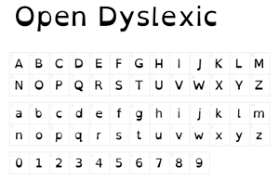
\includegraphics[width=1\linewidth]{open_dyslexic.png}
    \caption{OpenDyslexic Typeface \cite{13}}
    \label{fig:opendyslexic}
\end{figure}
\subsection{Vision-Based and Behavioral Screening Methods}
Vision-based approaches explore dyslexia through the lens of visual attention and oculomotor behavior, grounded in theories such as the magnocellular deficit \cite{4}. Eye-tracking studies reveal that readers with dyslexia exhibit distinct behavioral markers, including longer fixation durations, unstable gaze, and increased regression frequencies (backward eye movements) \cite{8}. Despite their predictive power, these systems typically require specialized hardware and operate as standalone screening tools rather than integrated, real-time assistive devices.

\subsection{The Need for Multimodal Integration}
Comprehensive reviews of assistive technologies highlight a persistent fragmentation in the field \cite{9}. Most tools prioritize a single modality, making it difficult to contextualize reading difficulty comprehensively. This separation leaves a gap for a system that can combine typographic accessibility with behavioral observation.



% ==========================
% SECTION III: PROBLEM FORMULATION
% ==========================
\section{Problem Formulation}

Despite the availability of diverse dyslexia technologies, their isolated deployment limits their overall effectiveness. Because dyslexia is a multidimensional neurocognitive condition, reading difficulty manifests differently across individuals and contexts. 

The current landscape suffers from two primary limitations:
\begin{itemize}
    \item \textbf{Disjointed Workflows:} The reliance on single-modality systems forces users to juggle disparate tools, increasing cognitive and operational burden rather than alleviating it.
    \item \textbf{Static Assistance:} Existing tools (e.g., standard text-to-speech or static fonts) act as passive filters. They do not actively observe user behavior to identify where cognitive friction occurs.
\end{itemize}

To address these challenges, an assistive reading environment must move beyond static text rendering. We propose that a modern dyslexia support system must meet three structural requirements:
\begin{enumerate}
    \item \textbf{Non-Intrusive Perceptual Assistance:} It must provide visual and auditory support that reduces cognitive load without mutating or permanently altering the underlying document text.
    \item \textbf{Word-Level Structural Awareness:} It must possess the architectural capacity to map interactions (such as caret position, scroll behavior, and eventual gaze tracking) to specific words in real-time.
    \item \textbf{Dynamic Difficulty Prediction:} It must leverage these behavioral and lexical signals to estimate cognitive load, transitioning from a reactive accessibility tool to a proactive, adaptive support system.
\end{enumerate}

The direct mapping between the limitations of traditional systems and these proposed structural requirements is summarized in Table~\ref{tab:requirements}.

\begin{table}[htbp]
\caption{Mapping Traditional Limitations to Synapse Architectural Requirements}
\centering
\begin{tabular}{|p{4cm}|p{4cm}|}
\hline
\textbf{Traditional System Limitation}
 & \textbf{Synapse Architectural Requirement} \\
\hline
Disjointed workflows across isolated, single-modality tools &
Unified, frontend-first multimodal integration \\
\hline
Permanent mutation of underlying text (e.g., destructive formatting) &
Non-intrusive, state-driven perceptual overlays \\
\hline
Inability to measure interaction at the granular word level &
Structural word-level awareness via tokenized DOM \\
\hline
Static, reactive accessibility filters &
Dynamic cognitive difficulty prediction (ML-driven) \\
\hline
Privacy risks associated with remote biometric processing &
Local, browser-based behavioral feature extraction \\
\hline
\end{tabular}
\label{tab:requirements}
\end{table}

% ==========================
% SECTION IV: UNIFIED SYSTEM ARCHITECTURE
% ==========================
\section{Unified System Architecture}

The Synapse framework is designed as a frontend-heavy, real-time assistive platform rather than a traditional, backend-dependent text processor. The architecture prioritizes low-latency visual control, reading flow preservation, and privacy-centric interaction analytics.

\subsection{Architectural Design Principles}
The system architecture was constructed around three core principles designed to address the fragmented nature of traditional dyslexia supports:
\begin{itemize}
    \item \textbf{Frontend-First Execution:} All real-time behavior, perception layers, and interaction tracking occur directly within the browser. This ensures sub-50\,ms latency for accessibility features and preserves user privacy.
    \item \textbf{State-Driven Rendering:} The architecture relies on centralized state management rather than event-driven backend workflows. The application controller manages settings, content, and session states, broadcasting these as dynamic styling properties to the view layer.
    \item \textbf{Decoupled Persistence:} Backend infrastructure is strictly utilized for persistence rather than active processing, ensuring the tool remains functional even in low-bandwidth educational environments.
\end{itemize}

\subsection{High-Level Technology Stack}
As illustrated in Fig.~\ref{fig:architecture}, the system is structured as a serverless web application. The frontend is developed using React with TypeScript to ensure type safety and manageable state, while Tailwind CSS handles layout structure.

\begin{figure}[htbp]
    \centering
    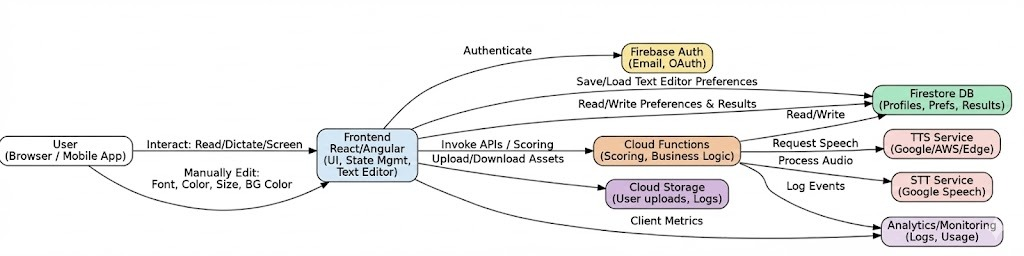
\includegraphics[width=1\linewidth]{b5346554-dc3b-4810-a99f-a5d80418a14f.jpg}
    \caption{High-level unified architecture illustrating the interaction between the frontend state controller, the reading interface, and the Supabase persistence layer.}
    \label{fig:architecture}
\end{figure}

The application state is centralized in a master controller, which serves as the single source of truth for user preferences, session tracking, and document content. The backend utilizes Supabase (PostgreSQL) for secure, anonymous synchronization of reading configurations and text documents.

\subsection{Structural Word-Level Awareness}
A critical architectural shift from traditional text editors is the abandonment of standard \texttt{<textarea>} inputs. Synapse utilizes a tokenized \texttt{contentEditable} surface. Upon ingestion, text is tokenized and every word is wrapped in an individual \texttt{<span>} element.

This DOM-level structural awareness enables precise programmatic control without mutating the underlying text. Words become individually addressable, establishing the necessary foundation for caret-to-word mapping, scroll-based focus detection, and future integration with webcam-based gaze tracking.

\subsection{State Management and Persistence Synchronization}
The architecture utilizes a unidirectional data flow governed by the central \texttt{App.tsx} controller. To minimize friction for users with cognitive disabilities, the system abandons traditional authentication barriers. Instead, a unique \texttt{session\_id} is generated via the browser's \texttt{localStorage} upon initialization. This session token acts as the primary foreign key for the Supabase PostgreSQL backend. 

When a user modifies a visual parameter via the control panel—such as shifting from standard spacing to a dyslexia-optimized layout—the state mutation triggers a React re-render. Simultaneously, a debounced asynchronous synchronization function pushes the updated configuration payload to the \texttt{user\_preferences} table. This ensures that the user's highly specific perceptual settings are instantly available upon their next session without requiring a login workflow.

\subsection{Document Ingestion and the PDF Parsing Pipeline}
A critical requirement for an assistive reader is the ability to ingest external academic and professional documents. PDF parsing is notoriously difficult in browser environments due to thread blocking. Synapse addresses this by implementing a dedicated Web Worker pipeline utilizing the \texttt{pdfjs-dist} library \cite{19}. 

When a user uploads a document, the file is handed off to a Vite-configured background worker (\texttt{pdfParser.ts}). The worker iterates through the document, extracting text layers page by page while discarding complex vector graphics and embedded images that cannot be parsed into the \texttt{contentEditable} surface. The extracted raw string is then passed back to the main thread, where the tokenization engine splits the string into individual word spans before injecting it into the React state. If the PDF consists of flattened images (lacking a selectable text layer), the pipeline catches the null return and triggers a graceful UI fallback.


% ==========================
% SECTION V: ASSISTIVE READER SYSTEM
% ==========================
\section{Assistive Reader System}

The core functional contribution of this work is the implementation of the Assistive Reader. The reader acts as a perceptual overlay engine that responds to user interaction dynamically.

\subsection{Visual Assistance Layers and Typography}
Rather than relying on static CSS classes, the editor calculates a \texttt{React.CSSProperties} object dynamically based on the state. This enables continuous, fine-grained control over typography. The system integrates the \textbf{OpenDyslexic} typeface, featuring weighted letter bases designed to reduce perceived character rotation and inversion \cite{13}.

The reader implements three distinct perceptual layers to reduce cognitive load:
\begin{itemize}
    \item \textbf{Reading Guide:} A dynamic horizontal overlay tracking the Y-axis of the user's cursor. This acts as a digital reading ruler to prevent line-skipping and loss of vertical tracking.
    \item \textbf{Focus Mode:} Absolute-positioned gradient masks that dim the surrounding text above and below the active reading area, simulating a "tunnel vision" effect to reduce visual clutter and peripheral distraction.
    \item \textbf{Word Highlighting:} Dynamic CSS adjustments that increase inter-word spacing and apply distinct selection contrast, preventing words from crowding together visually (the "crowding effect").
\end{itemize}

\begin{figure}[htbp]
    \centering
    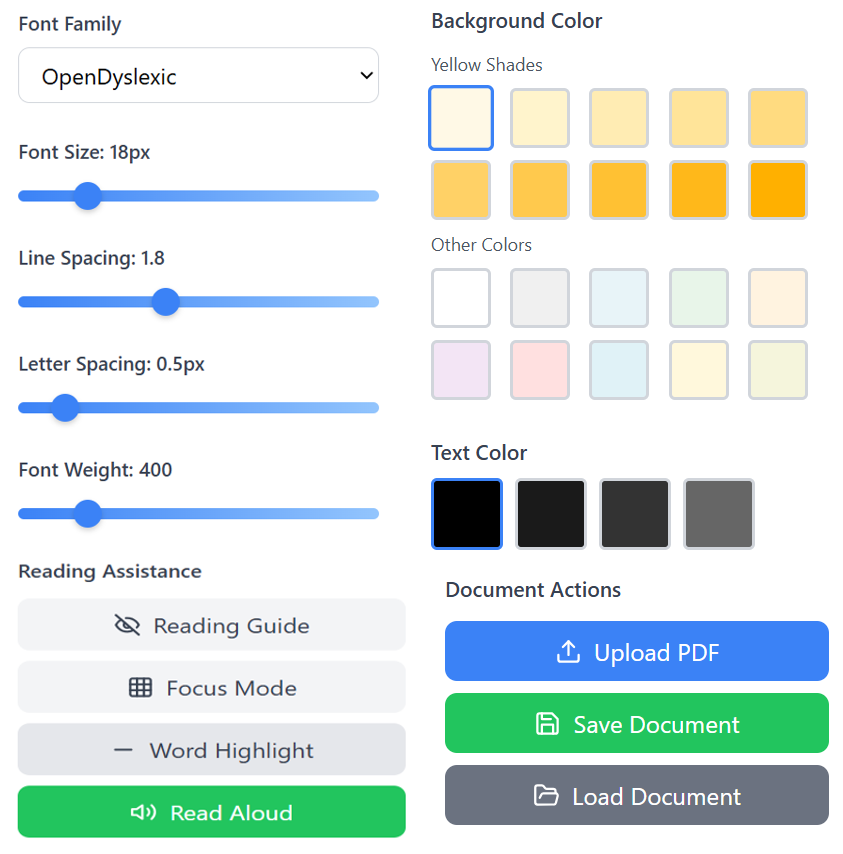
\includegraphics[width=0.8\linewidth]{2x2.png}
    \caption{\textbf{Implemented Assistive Interface.} (a) Sidebar control panel for granular typography adjustment. (b) Central reading pane with active karaoke-style highlighting using the OpenDyslexic typeface. (c) ``Yellow Mode'' display to reduce visual stress.}
    \label{fig:reader_ui}
\end{figure}

\subsection{Therapeutic Mechanisms and Cognitive Support}
By abandoning the standard text editor model in favor of a tokenized reading surface, the Assistive Reader provides support across three scientifically grounded cognitive dimensions:
\begin{enumerate}
    \item \textbf{Bi-Modal Reinforcement (Phonological Support):} Dyslexia is strongly associated with difficulty mapping phonemes to graphemes \cite{3}. By highlighting individual word tokens synchronously as they are spoken, the system actively tries reinforcing and may assist the cognitive connection between auditory sound and visual spelling.
    \item \textbf{Oculomotor Guidance:} Readers with dyslexia frequently exhibit involuntary backward eye movements (regressions) during reading \cite{8}. The synchronized visual highlighter serves as a forward-moving anchor that guides visual attention, reducing the frequency of backward skips.
    \item \textbf{Working Memory Offloading:} When decoding demands are high, working memory resources are often diverted away from reading comprehension \cite{14}, \cite{15}. By shifting the decoding burden to the automated Text-to-Speech audio, the system preserves working memory capacity, allowing users to concentrate purely on grasping the narrative content.
\end{enumerate}

\subsection{Scroll Architecture and Stability}
To accommodate lengthy documents, the application layout is scroll-locked. The main body of the application remains fixed, while the editor container handles its own internal scrolling. This guarantees that the control panel and visual assistance overlays remain perfectly aligned, and that low-contrast background colors (such as the default \#FFF9E6 yellow shade, known to alleviate visual stress \cite{6}) do not clip or disappear during document navigation. These are constrained to maintain contrast ratios compliant with standard Web Content Accessibility Guidelines (WCAG) as well.

\subsection{Dual-Mode Text-to-Speech and Document Ingestion}
To provide continuous auditory reinforcement without blocking browser rendering threads, the system employs a dual-mode TTS engine using the native \texttt{SpeechSynthesisUtterance} API. Large texts are split into sentence or paragraph chunks prior to playback, eliminating preprocessing delays and allowing smooth, sequential reading of full documents. Alternatively, users can highlight specific phrases to trigger isolated TTS playback (Speak Selection), enabling micro-level auditory support for particularly challenging passages.
\subsection{Algorithmic Tokenization for DOM Mapping}
The transition from a standard \texttt{<textarea>} to a \texttt{contentEditable} surface requires a robust tokenization algorithm. In standard text inputs, measuring the exact screen coordinates of a specific word is computationally prohibitive. Synapse solves this by intercepting the ingested text and applying a regular expression-based tokenizer that splits the document at word boundaries and whitespace characters. 

Each token is then wrapped in a standard HTML \texttt{<span>} tag with a dedicated \texttt{data-word="true"} attribute. This structural injection transforms a flat string into a queryable DOM tree. Consequently, the system can utilize the \texttt{getBoundingClientRect()} API to calculate the exact X and Y coordinates of any given word. This architectural foundation is what makes the dynamic Reading Guide possible, and it serves as the critical prerequisite for mapping webcam gaze vectors to specific words in future iterations.

\subsection{Chunking Heuristics for Text-to-Speech (TTS)}
Native browser implementations of the \texttt{SpeechSynthesisUtterance} API frequently suffer from buffer overloads and significant latency when presented with large text blocks. To guarantee low-latency auditory feedback, Synapse employs a chunking heuristic. 

Before playback, the active document is algorithmically partitioned into sentence or paragraph blocks using punctuation delimiters. The TTS engine queues these chunks sequentially. As the API emits an \texttt{onboundary} event during playback, the application state updates, instantly applying a CSS highlight class to the corresponding \texttt{<span>} element. This chunked architecture ensures that a 50-page PDF begins playback with the same sub-50\,ms latency as a single-paragraph document.


% ==========================
% SECTION VI: EXPERIMENTAL RESULTS
% ==========================
\section{Experimental Results: Cognitive Difficulty Prediction}

To transition Synapse from a reactive accessibility tool to an adaptive system, we developed a machine learning pipeline capable of predicting word-level cognitive load. By estimating reading difficulty dynamically, the system can eventually adjust perceptual overlays based on predicted friction points.

\subsection{Dataset and Target Variable Formulation}
Model training and evaluation were conducted using the Zurich Cognitive Language Processing Corpus (ZuCo) \cite{16}. We merged data from both the L1 and L2 reading tasks to create a comprehensive baseline. 

Because cognitive load is subjective and lacks a discrete binary label in raw eye-tracking data, we engineered a ground-truth target variable ('is\_difficult'). First, the raw gaze metrics were z-score normalized to account for baseline reading speed differences across subjects. We then calculated a composite ``stress score'' by aggregating the median normalized gaze features for each word. Words falling into the top quartile (the 75th percentile, $\ge 0.75$ quantile) of this stress score were labeled as cognitively difficult (Class 1), while the remainder were labeled as baseline (Class 0).

\subsection{Psycholinguistic Feature Engineering}
We extracted two primary feature sets for each word token:
\begin{itemize}
    \item \textbf{Lexical Features:} Character length (\texttt{char\_len}), syllable count (approximated via a localized regex heuristic isolating vowel groupings, \texttt{[aeiouy]+}), and vowel ratio (\texttt{vowel\_ratio}). 
    \item \textbf{Gaze/Behavioral Features:} Total reading time (\texttt{word\_total\_reading\_time}), go-past time (\texttt{word\_go\_past\_time}), first fixation duration (\texttt{word\_first\_fixation\_duration}), and gaze duration (\texttt{word\_gaze\_duration}). Missing gaze values—often resulting from hardware tracking loss—were imputed using median values for continuous features.
\end{itemize}

\subsection{Algorithmic Selection and Hardware Environment}
We selected tree-based ensemble models due to their ability to handle non-linear feature interactions and their native compatibility with SHAP explainability matrices \cite{18}. The experimental pipeline was executed in a GPU-accelerated environment utilizing a Kaggle Nvidia P100 GPU instance.

The hyperparameter configurations for the tested models were explicitly tuned for this tabular dataset:
\begin{itemize}
    \item \textbf{Random Forest:} 500 estimators, balanced class weights, utilizing all available CPU cores (\texttt{n\_jobs=-1}).
    \item \textbf{Gradient Boosting:} 300 estimators, learning rate of 0.05.
    \item \textbf{XGBoost \cite{17}:} 800 estimators, max depth of 6, learning rate of 0.03, utilizing a histogram-based tree method (\texttt{tree\_method="hist"}) mapped directly to the CUDA device for hardware acceleration. Subsample and column-sample by tree were both constrained to 0.8 to prevent overfitting.
\end{itemize}

\subsection{Cross-Validation Strategy and Ablation Study}
To rigorously prevent data leakage, we employed a \texttt{GroupKFold} cross-validation strategy ($K=5$). The folds were grouped by subject ID (\texttt{pp\_nr}), ensuring that a single participant's reading patterns did not appear in both the training and testing splits simultaneously. 

We conducted an ablation study across three configurations: Lexical-only, Gaze-only, and Combined features. The consolidated results are presented in Table~\ref{tab:ablation_results}.

\begin{table}[htbp]
\caption{Ablation Study Results (5-Fold Grouped CV Means)}
\centering
\begin{tabular}{|l|l|c|c|}
\hline
\textbf{Feature Set} & \textbf{Model} & \textbf{Mean AUC} & \textbf{Mean F1} \\
\hline
\multirow{3}{*}{Lexical Only} 
 & Random Forest & 0.6430 & 0.4254 \\
 & Gradient Boosting & 0.6432 & 0.0751 \\
 & XGBoost & 0.6432 & 0.0724 \\
\hline
\multirow{3}{*}{Gaze Only} 
 & Random Forest & 0.9979 & 0.9795 \\
 & Gradient Boosting & 0.9983 & 0.9775 \\
 & XGBoost & 0.9988 & 0.9805 \\
\hline
\multirow{3}{*}{Combined} 
 & Random Forest & 0.9985 & 0.9798 \\
 & Gradient Boosting & 0.9983 & 0.9774 \\
 & \textbf{XGBoost} & \textbf{0.9989} & \textbf{0.9804} \\
\hline
\end{tabular}
\label{tab:ablation_results}
\end{table}

\subsection{Interpretation of Predictive Performance}
The ablation results demonstrate a stark contrast between feature sets. Lexical-only models performed poorly, achieving a maximum Mean AUC of ~0.643. Conversely, the Gaze-only models exhibited massive predictive dominance, pushing the Mean AUC to ~0.998. When both feature sets were combined, the XGBoost model achieved the highest overall performance (AUC: 0.9989, F1: 0.9804). This confirms our architectural hypothesis: cognitive difficulty is primarily a perceptual and behavioral phenomenon, and assistive systems must observe user interaction rather than relying solely on static text analysis.

\subsection{Feature Importance and Explainability}
To ensure the model's predictions remain interpretable for educational and clinical contexts, we applied SHapley Additive exPlanations (SHAP) \cite{18} to the XGBoost Combined model via the \texttt{TreeExplainer} API. 

\begin{figure}[htbp]
    \centering
    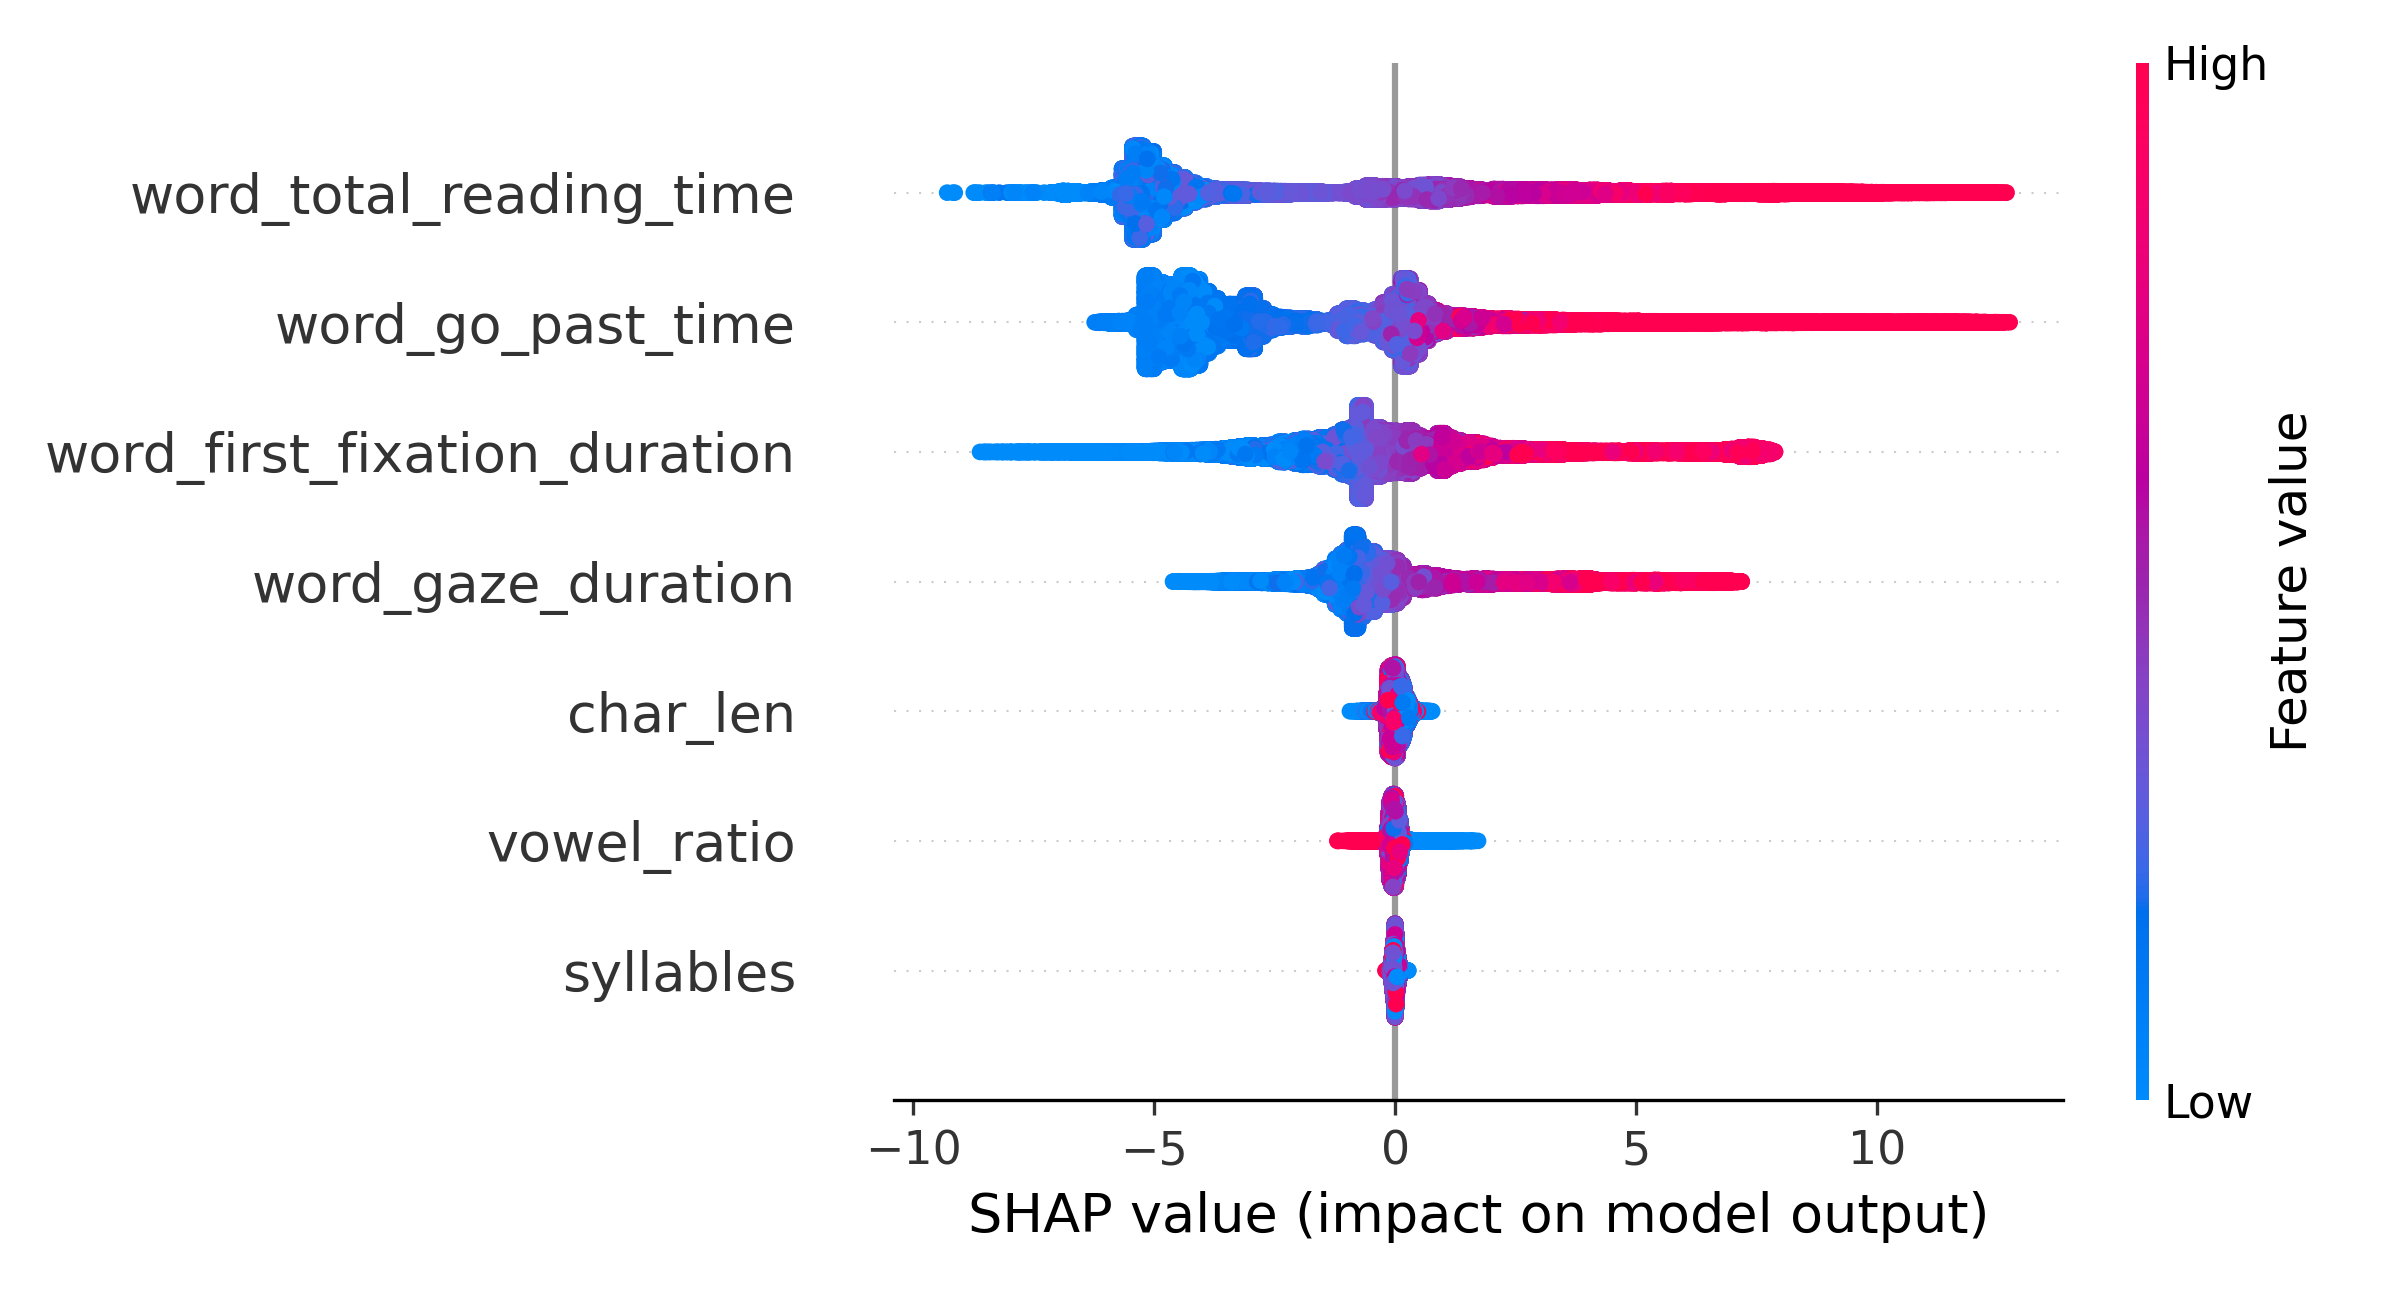
\includegraphics[width=1\linewidth]{shap_summary.png}
    \caption{SHAP summary plot illustrating feature impact on model output. Gaze features heavily dominate the predictive logic, while lexical features provide minor secondary signals.}
    \label{fig:shap_analysis}
\end{figure}

As shown in Fig.~\ref{fig:shap_analysis}, behavioral gaze metrics—specifically \texttt{word\_total\_reading\_time} and \texttt{word\_go\_past\_time}—are the most influential features. High values in these features strongly push the model toward predicting high cognitive difficulty. In contrast, lexical features like \texttt{char\_len} and \texttt{vowel\_ratio} cluster near the zero-impact baseline. However, their inclusion remains valuable for edge cases where behavioral signals may be temporarily noisy.

% ==========================
% SECTION VII: DISCUSSION, LIMITATIONS, AND FUTURE WORK
% ==========================
\section{Discussion, Limitations, and Future Work}

The transition from a static reading interface to an adaptive, machine-learning-driven environment introduces new opportunities for personalized dyslexia support, alongside distinct technical and ethical challenges.

\subsection{Privacy and Data Governance}
When developing technologies that capture behavioral or biometric data, privacy and data governance are paramount. Synapse addresses this through its frontend-first architecture. By processing behavioral signals (such as caret tracking and scroll velocity) locally within the browser, the system avoids transmitting raw interaction data to remote servers. Any future cloud-based ML processing will rely exclusively on anonymized, encoded feature vectors, aligning with strict educational data protection regulations. 

\subsection{Generalization Across Linguistic Contexts}
Dyslexia manifests differently across languages, as shallow orthographies emphasize phonological decoding while deep orthographies increase visual processing demands. Synapse’s modular architecture supports cross-linguistic generalization by allowing accessibility features and behavioral models to be recalibrated for specific orthographic contexts without altering the core engine.

\subsection{Limitations: The Webcam Tracking Gap}
Our experimental results indicate that gaze-based features heavily dominate cognitive load prediction. However, the ZuCo dataset relies on clinical-grade, infrared eye-tracking hardware. Translating these results to consumer-grade hardware presents a significant limitation. 
During initial system prototyping, we evaluated CNN-based gaze estimation pipelines using OpenFace \cite{19} (incorporating MTCNN \cite{20} for face detection and CLNF \cite{21} for landmark extraction). However, the computational overhead and latency of running real-time Perspective-n-Point (PnP) head pose estimation proved prohibitive for a lightweight, serverless browser architecture. While the Synapse framework mitigates some of this by tracking DOM-based behavioral cues rather than seeking millimeter level precision, current ML model accuracy will likely degrade when applied to noisy, real-world webcam feeds. This computational bottleneck justifies our future transition toward lightweight, browser-native face meshes (e.g., MediaPipe).

\subsection{Future Research Roadmap}
To bridge the gap between our current baseline and a fully adaptive reading engine, future work is structured across three phases:
\begin{enumerate}
    \item \textbf{Behavioral Signal Integration:} Before deploying webcam gaze tracking, we will integrate highly reliable, DOM-based behavioral signals—such as caret dwell time, scroll pauses, and TTS replay frequency. These metrics will serve as proxy indicators for visual attention and cognitive friction.
    \item \textbf{Webcam-Based Gaze Estimation:} We plan to integrate browser-based gaze estimation (e.g., using MediaPipe FaceMesh) to map approximate gaze coordinates to our tokenized \texttt{contentEditable} word bounding boxes, combining gaze and caret data for higher confidence.
    \item \textbf{The Adaptive Reading Engine \& Longitudinal A/B Testing:} Ultimately, predicted difficulty scores will trigger real-time UI adaptations. Instead of static settings, the system will dynamically adjust font weight, increase word spacing, or alter TTS pacing exclusively for sentences predicted to induce high cognitive load. To validate these adaptive UI changes, planned longitudinal A/B studies will evaluate user performance against traditional text interfaces. Evaluation will track changes in words per minute (WPM), reading accuracy, and comprehension retention over extended periods to ensure multimodal cues provide enduring cognitive benefits.
\end{enumerate}

% ==========================
% SECTION VIII: CONCLUSION
% ==========================
\section{Conclusion}

Current dyslexia support technologies frequently force users to choose between isolated tools—such as standalone text-to-speech software, static typography adjustments, or clinical gaze-tracking screenings. This fragmentation results in a reactive approach to accessibility, where systems cannot dynamically respond to a reader's cognitive state.

In this paper, we presented Synapse, a multimodal assistive reading system that bridges the gap between typographic accessibility and behavioral observation. By shifting from a standard text input to a tokenized \texttt{contentEditable} surface, we established a structurally aware architecture capable of mapping user interaction at the word level. Furthermore, our evaluation using the ZuCo dataset confirms that behavioral signals—specifically reading and gaze durations—are vastly superior to lexical features in predicting cognitive difficulty, achieving an AUC of 0.9989 using XGBoost.

Synapse does not merely render text; it observes how that text is consumed. By combining a privacy-first, serverless frontend with a robust machine learning pipeline, this system provides a foundation for proactive, personalized reading support that adapts to the user in real-time.

\section*{Data and Code Availability}
The Zurich Cognitive Language Processing Corpus (ZuCo) utilized for the machine learning evaluation in this study is a publicly available dataset. The implementation code for the Synapse frontend architecture, the tokenization engine, and the XGBoost predictive modeling pipeline will be made available in a public repository upon publication to support reproducibility and further research in accessible computing.
% ==========================
% REFERENCES
% ==========================
\begin{thebibliography}{00}

\bibitem{1}
D. L. Lefly and B. F. Pennington,
``Reliability and validity of the Adult Reading History Questionnaire,''
\textit{Journal of Learning Disabilities}, vol. 33, no. 3, pp. 286--296, 2000.

\bibitem{2}
A. J. Fawcett and R. I. Nicolson,
\textit{Dyslexia Screening Test (DST)},
London, U.K.: Harcourt Assessment, 1996.

\bibitem{3}
M. J. Snowling,
\textit{Dyslexia},
Oxford, U.K.: Blackwell Publishing, 2000.

\bibitem{7}
E. L. F. da Silva, R. S. Guti\'errez, and A. P. C. da Silva,
``Using acoustic features to identify speech difficulties associated with dyslexia,''
\textit{International Journal of Speech Technology}, vol. 22, pp. 601--612, 2019.

\bibitem{10}
E. L. F. da Silva \textit{et al.},
``Automatic detection of reading difficulties using speech alignment patterns,''
in \textit{Proc. IEEE Int. Conf. Acoustics, Speech and Signal Processing (ICASSP)},
2021, pp. 7428--7432.

\bibitem{12}
S. Cox and S. Dasmahapatra,
``High-level approaches to confidence estimation in speech recognition,''
\textit{IEEE Transactions on Speech and Audio Processing}, vol. 10, no. 7, pp. 460--471, 2002.

\bibitem{14}
A.~D. Baddeley and G.~Hitch,
``Working Memory,''
\textit{Psychology of Learning and Motivation},
vol.~8, pp.~47--89, 1974.

\bibitem{15}
J.~Sweller,
``Cognitive load during problem solving: Effects on learning,''
\textit{Cognitive Science},
vol.~12, no.~2, pp.~257--285, 1988.

\bibitem{6}
H. Irlen,
\textit{Reading by the Colors: Overcoming Dyslexia and Other Reading Disabilities Through the Irlen Method},
New York, NY, USA: Avery Publishing, 2005.

\bibitem{5}
S. N. Abdul Wahid,
``Evaluation of dyslexia-friendly fonts for improved readability,''
\textit{International Journal of Education and Literacy}, 2017.

\bibitem{13}
A. Gonzalez,
``OpenDyslexic: A typeface for dyslexia,''
OpenDyslexic, 2011. [Online]. Available: \url{https://opendyslexic.org}

\bibitem{4}
J. Stein,
``The magnocellular theory of developmental dyslexia,''
\textit{Dyslexia}, vol. 7, no. 1, pp. 12--36, 2001.

\bibitem{8}
M. N. Benfatto \textit{et al.},
``Screening for dyslexia using eye tracking during reading,''
\textit{Journal of Learning Disabilities}, vol. 49, no. 2, pp. 196--208, 2016.

\bibitem{9}
A. Khalid, M. Zaffar, and M. Ramzan,
``Assistive technologies for dyslexia: A review,''
\textit{IEEE Access}, vol. 8, pp. 64589--64609, 2020.

\bibitem{19}
Mozilla Foundation, 
``PDF.js: A General-Purpose, Web Standards-Based Platform for Parsing and Rendering PDFs,'' 
2024. [Online]. Available: https://mozilla.github.io/pdf.js/

\bibitem{16}
N. Hollenstein et al., 
``ZuCo, a simultaneous EEG and eye-tracking resource for sentence reading,'' 
\textit{Scientific Data}, vol. 5, no. 1, pp. 1--13, 2018.

\bibitem{18}
S. M. Lundberg and S.-I. Lee, 
``A Unified Approach to Interpreting Model Predictions,'' 
in \textit{Advances in Neural Information Processing Systems (NeurIPS)}, vol. 30, 2017.

\bibitem{17}
T. Chen and C. Guestrin, 
``XGBoost: A Scalable Tree Boosting System,'' 
in \textit{Proc. 22nd ACM SIGKDD International Conference on Knowledge Discovery and Data Mining}, 2016, pp. 785--794.
\bibitem{19} T. Baltrušaitis, P. Robinson, and L.-P. Morency, "OpenFace: an open source facial behavior analysis toolkit," in \textit{IEEE Winter Conference on Applications of Computer Vision (WACV)}, 2016, pp. 1--10.
\bibitem{20} K. Zhang, Z. Zhang, Z. Li, and Y. Qiao, "Joint face detection and alignment using multitask cascaded convolutional networks," \textit{IEEE Signal Processing Letters}, vol. 23, no. 10, pp. 1499--1503, 2016.
\bibitem{21} T. Baltrušaitis, P. Robinson, and L.-P. Morency, "Constrained Local Neural Fields for robust facial landmark detection in the wild," in \textit{IEEE International Conference on Computer Vision Workshops (ICCVW)}, 2013, pp. 354--361.
\end{thebibliography}



\end{document}
